\documentclass[tcn = 45538, sheet = true, abstract = true]{mcmthesis}
\problem{E}
\usepackage{palatino}
\usepackage{mwe}
\usepackage{booktabs}
\title{Analysis and Optimization of Water Resources: with India for example}
\author{45538}
\date{\today}

\begin{document}

\begin{titlepage}
\begin{abstract}

Providing a water resources strategy for the International Clean water Movement 
(ICM) 
poses a severe challenge. 
World is experiencing its severe water shortage, 
while we need to make more use of what we have.
Thus, 
understanding the changes of water resources is greatly helpful 
in analyzing the impacts of environmental and social drivers, 
formulating plans for utilization of water resources,
and generating water resource strategy.

This paper explores the method of comprehensive evaluation of water resources providing ability, 
and sets up an evaluation model applying the fuzzy comprehensive evaluation method. 
Built on the data of domestic, industrial, agriculture use of water resources in India, 
we evaluate the water resources providing ability of India by means of the model. 

Using authoritative history data, 
we use Grey Prediction Model to assist in predicting total demand for water through a statistical view
and establish the Logistic Retarded Growth Model to predict the population in India in 15 years.

Considering limited water resources and inadequate sewage disposal systems, 
we design a sensible intervention plan. 
By using applied mathematics method, 
we establish the Sewage Disposal Price System, 
Sewage Disposal Quantity System and Psychological Prediction Model to discuss the impact on the surrounding areas, 
as well as the entire water ecosystem.

Through our models, 
water will become a critical issue in India around 2017 with no intervention, 
while water scarcity will be postponed by 2 years with our intervention. 
If water resources exploitation extent reaches 90\% in India, 
this severe problem won't happen until 2024.

\begin{keywords}
water resources; 
India; 
Grey Forecasting Model; 
Logistic Retarded Growth Model
\end{keywords}

\end{abstract}

\maketitle
\end{titlepage}
\newpage

\tableofcontents
\newpage

\section{Introduction}

\hspace{1.5 em} Last year witnessed \emph{The Drinkable Book} made the headlines - 
this new technology has been tested with over 25 different water sources in 5 countries, 
and they are starting to pilot in a few villages in Africa and Asia. 
\emph{"They've completed an important step and there are more to go through."} 
Dr Lantagne said. 
Our group wants to try our best to help solve the world's water problem.

Water is the source of life. 
It is a critical natural resource upon which all social and economic activities and ecosystem functions depend. 
As it's known to all, world's fresh water resource situation is not optimistic, 
and there are two primary causes at present. 
One is environmental (physical) scarcity, 
and the other one is social (economic) scarcity. 
One must not only understand the environmental constraints on water supply, 
but also how social factors influence availability and distribution of clean water. 

\subsection{Precondition}
\label{precondition}

\hspace{1.5 em} Water resources development and utilization are the activity of planning, 
developing, distributing and managing the use of water resources. 
It is a sub-set of water cycle management.
\footnote{Wikipedia, the free encyclopedia. 
Water resource management. 
\emph{Wikipedia}, 
January 2016.}
Ideally, water resources development and utilization quotiety are expected to be almost stable.

Another aspect regarding to our issue is the demand for water. 
Mainly, water requirement comes from primary (agriculture), 
secondary (production and construction), 
and tertiary (service)
sector of the economy, 
ecological environment and domestic. 
The water consumption of tertiary industry and ecological environment consumption account for less than 1 per cent of the total demand, 
thus could be disregarded, 
which leaves 3 major influencing factors. 
Domestic demand is equivalent to the product of water demand per capita, 
and the population. 
Gross domestic product (GDP) 
is a monetary measure of the value of all final goods and services produced in a period 
(quarterly or yearly).
\footnote{Wikipedia, the free encyclopedia. 
Gross domestic product. 
\emph{Wikipedia}, 
January 2016.}
In our case, 
we take agriculture and industry into account. 

\subsection{Parameters}

\hspace{1.5 em} Parameters involved in this model are shown as follows:

\begin{itemize}
\item Quantity of a region's water resources $\alpha$
\item Quantity of sewage $\beta$
\item Water resources utilization level $\lambda$
\item Water resources exploitation extent $\mu$
\item Supply of water $\gamma$
\item Industrial water requirement $\omega$
\item Agricultural water consumption $\varphi$
\item Water demand per capita $\varepsilon$
\item Population $\theta$
\item Relation between water supply and demand $\rho$
\end{itemize}

\subsection{Evaluation Model}

\qquad We can get $\alpha$ by look-up table, which is related to the region; 
we can also obtain $\beta$ by look-up table, which is a social factor;  
we assume that the social factor $\lambda$ and $\mu$ are constant values. 
Considering $\alpha$ refers to quantity of a region's water resources, 
while $\beta$ refers to the quantity of sewage, 
we have $\gamma$, the social factor 
\begin{equation}
\gamma = \alpha \cdot \lambda \cdot \mu - \beta
\label{eq:supply}
\end{equation}

$\omega$ are social factors connected with economic development; 
we can get $\varepsilon$ by look-up table, 
which is connected with the environment as well as the economic development of the region; 
$\theta$ can also be got by look-up table.

Several parameters are related to time, which are $\beta$, $\omega$, $\varphi$, $\varepsilon$ and $\theta$.

According to the parameters shown above, we have the model
\begin{equation}
\rho = \frac{\gamma}{\omega + \varphi + \varepsilon \cdot \theta }
\label{eq:relation}
\end{equation}

The increasing of $\rho$ indicates that the region excessively supplies clean water; 
and vice versa.

\section{Analysis of India water scarcity}

\hspace{1.5 em} Clean water is so desperately needed in India. 
The Analysis of Indian water scarcity is the test of our model. 
We pick India whose water is moderately overloaded. 
And explain both the environmental and social drivers of this status.

\subsection{Results Of Evaluation Model}

\hspace{1.5 em} As with Table \ref{tab:waterConditionOfIndia}
\footnote{UN FAO, AQUASTAT database. 
Food and Agriculture Organization of the United Nations. 
2013.}
\footnote{Wikipedia, the free encyclopedia. 
Water pollution in India Water pollution in India. 
\emph{Wikipedia}, 
December 2015.}
, this table on water condition of India has appeared in some form. 

\begin{table}[]
\centering
\begin{tabular}{@{}c|c|c@{}}
\toprule
Parameter & Value & Unit \\ \midrule
$\alpha$ & 1,911.0 & $km^3/yr$ \\
$\beta$ & 13.99921 & $km^3/yr$ \\
$\omega / \theta$ & 14 & $m^3/p/yr$ \\
$\varphi / \theta$ & 567 & $m^3/p/yr$ \\
$\varepsilon$ & 46 & $m^3/p/yr$ \\
$\theta$ & 1,214.46 & millions \\ \bottomrule
\end{tabular}
\caption{Water condition of India}
\label{tab:waterConditionOfIndia}
\end{table}

The quantity of water in India could supply every year $\gamma$ like Equation \eqref{eq:supply}. 
Through searching the related resources data, 
we have $\lambda = 60.0\%$,  
$\mu = 53.6\%$, 
thus, supply of water $\gamma = 600.578 km^3/yr$.

The same procedure may be easily adapted to obtain our models for other state parameters,
which means $\rho$ = 78.887\%.

\subsection{Explanation On Evaluation Model}

\hspace{1.5 em} Depending on the result of the Evaluation Model, 
water is heavily overloaded in India.
There is not sufficient water for all uses, 
whether agricultural, 
industrial or domestic. 
It has been proposed that when annual per capita renewable freshwater availability is less than 1,700 cubic meters, 
countries begin to experience periodic or regular water stress. 
Below 1,000 cubic meters, 
water scarcity begins to hamper economic development and human health and well-being. 
Unfortunately, 
this figure towards India is approximately 1,103 cubic meters, 
which is close to water scarcity warning line. 

\begin{itemize}
\item \textbf{Environmental drivers} \\

\emph{Geography} 

The Indian climate is heavily influenced by the Himalayas and the Thar Desert, 
both of which drive the economically and culturally pivotal summer and winter monsoons. 
The Himalayas prevent cold Central Asian katabatic winds from blowing in, 
keeping the bulk of the Indian subcontinent warmer than most locations at similar latitudes. 
The Thar Desert plays a bital role in attracting the moisture-laden south-west summer monsoon winds that, 
between June and October, provide the majority of India's rainfall. 
Four major climatic groupings predominate in India: 
tropical wet, 
tropical dry, 
subtropical humid, 
and montane. 

\emph{Climate change}

Climate change could have significant impacts on water resources in India because of the intimate connections between the climate and the hydrological cycle. 
Rising temperatures will increase evaporation and lead to increases in precipitation. 
Both droughts and floods may become more frequent in India. 
Possible impacts include increased eutrophication. 
Climate change could also mean an increase in demand for farm irrigation, 
garden sprinklers. 
There is currently ample evidence that increased hydrology variability and change in climate has and will continue to have a profound impact on the water sector through the hydrology cycle, 
water availability and water demand.

\item \textbf{Social drivers} \\

\emph{Population growth} 

The Indian population was 1295.29 million in 2014. 
Thus, 
water demand will increase unless there are corresponding increases in water conservation and recycling of this vital resource. 
Access to water for producing food will be one of the main challenges in the decade to come, 
which will need to be balanced with importance of managing water itself in a sustainable way, 
taking into account the impact of climate change and other environmental and social variables. 

\emph{Expansion of business activity} 

Business activity ranging from industrialization to services such as tourism and entertainment in India continues to expand rapidly. 
This expansion requires increased water services including both supply and sanitation, 
which can lead to more pressure on water resources and the natural ecosystem.

\emph{Depletion of aquifers}

Due to the expanding human population, 
competition for water is growing such that many of the world's major aquifers are becoming depleted. 
This is due both for direct human consumption as well as agricultural irrigation by groundwater. 

\emph{Pollution}

Water pollution is among the main concerns of India today. 
Many pollutants threaten water supplies, 
but the discharge of raw sewage into natural waters is the most common method in India. 
Sewage, 
sludge, 
garbage, 
and even toxic pollutants are all dumped into the water. 
Even if sewage is treated, 
problems still arise. 
In addition to sewage, 
non point source pollution such as agricultural runoff is a significant source of pollution in India, 
along with urban stormwater runoff and chemical wastes dumped by industries and governments.
\footnote{Wikipedia, the free encyclopedia. 
Water resources.  
\emph{Wikipedia}, 
February 2016.}

\end{itemize}

Given the seriousness of India water supply and demand imbalances, 
India is trapped in a vicious cycle of economic and social development 
- lacking degree of inadequacy of India water resources aggravation 
- water contradiction acute, 
with industrial and agricultural water requirement seize ecological environment water demand 
- ecological and environmental deterioration 
- vegetation degradation 
- economic and social development blocked. 
Water resources in India are scarce and systems for allocating water resources are scarce too.

\section{Grey Forecasting Model}

\hspace{1.5 em} What is happening in India, 
which has too many people in places where there is not enough water, 
is a foretaste of what is to come. 
In a thirsty region, 
prediction of water by 2031 is necessary for envisioning future scenarios and helping pro-active adaptation strategy. 

In this section, 
we make a prediction comprising total supply and demand tooling GM(1,1) and Logistic Retarded Growth Model.

\subsection{Assumptions}

\hspace{1.5 em} Based on Evaluation Model, 
the ratio of ability to provide clean water is for two figures to decide, 
which are the total supply and demand of water. 

\begin{itemize}

\item Water resources exploitation extent was stable in the recent past years. 
We assume it invariant, 
which leads total supply of water basically unchanged. 

\item As we said above in Section \ref{precondition}, 
non-domestic water supply is influenced by agricultural and industrial demand. 
We believe constant-price GDP is closely related to water consumption. 
That is non-domestic water supply equals divide constant-price GDP by water productivity. 

We mention seveval theorems here. 

\begin{Theorem}
Constant-price GDP also called real GDP; 
it is inflation-adjusted GDP. 
Constant-price GDP measures the value of a country's goods and services in relation to a base year. 
\footnote{Investing Answers. 
Constant-Price GDP. 
\emph{Financial Dictionary}, 
2016.}
\label{thm:constantPriceGDP}
\end{Theorem}

\begin{Theorem}
Inflation as measured by the annual growth rate of the GDP implicit deflator shows the rate of price change in the economy as a whole. 
The GDP implicit deflator is the ratio of GDP in current local currency to GDP in constant local currency.
\footnote{The World Bank. 
Inflation, GDP deflator (annual \%). 
\emph{World Development Indicators}, 
December 2015.}
\label{thm:inflationGDPDeflator}
\end{Theorem}

Table \ref{tab:inflationGDPDeflator}
\footnote{The World Bank. 
Inflation, GDP deflator (annual \%). 
\emph{World Development Indicators}, 
December 2015.}
is on inflation, 
GDP deflator of India.

\begin{table}[]
\centering
\begin{tabular}{@{}cc|cc|cc@{}}
\toprule
Year & \begin{tabular}[c]{@{}c@{}}Inflation\\ (annual \%)\end{tabular} & Year & Inflation & Year & Inflation \\ \midrule
1961 & 2.14542764259727 & 1962 & 4.40561674267815 & 1963 & 8.35362386003059 \\
1964 & 8.55167697678436 & 1965 & 8.30036942444605 & 1966 & 13.2707065560506 \\
1967 & 8.61620470798519 & 1968 & 2.41538358224665 & 1969 & 3.34336433990501 \\
1970 & 1.5622434894957 & 1971 & 5.32484104024424 & 1972 & 10.8396026988096 \\
1973 & 17.8297156461729 & 1974 & 16.6675157302367 & 1975 & -1.64868154554671 \\
1976 & 5.98185933336551 & 1977 & 5.6372293455353 & 1978 & 2.46028231547959 \\
1979 & 15.7280432071898 & 1980 & 11.5083208127639 &1981 & 10.8275819783816 \\
1982 & 8.09586309896582 & 1983 & 8.55285960515417 & 1984 & 7.92323284632677 \\
1985 & 7.19378544706504 & 1986 & 6.78940045157084 & 1987 & 9.3278933052373 \\
1988 & 8.23251536615848 & 1989 & 8.43680887306273 & 1990 & 10.6683038465274 \\
1991 & 13.7518189440416 & 1992 & 8.96515235934562 & 1993 & 9.86178285382972 \\
1994 & 9.98004477534052 & 1995 & 9.06270221988214 & 1996 & 7.57501828846144 \\
1997 & 6.47627126322838 & 1998 & 8.01016752360506 & 1999 & 3.06839552032511 \\
2000 & 3.644970161058 & 2001 & 3.21561601740324 & 2002 & 3.71568377657489 \\
2003 & 3.86779808618248 & 2004 & 5.72541322722107 & 2005 & 4.23692511895295 \\
2006 & 6.42259004900228 & 2007 & 5.75624346624512 & 2008 & 8.66466534681875 \\
2009 & 6.06382663975592 & 2010 & 8.9838126852477 & 2011 & 6.39886144585687 \\
2012 & 7.62581432706857 & 2013 & 6.25028547668308 & 2014 & 3.03592252416092 \\ \bottomrule
\end{tabular}
\caption{Inflation, GDP deflator of India}
\label{tab:inflationGDPDeflator}
\end{table}

Figure \ref{fig:inflationGDPDeflator} describes the inflation, GDP deflator of India. 
We can tell that GDP deflator has discrete variation, 
and a variety of factors involving thorny issues like world economy affect it, 
thus this index mark is among the hard-to-predict extreme ones. 
However, 
in recent years, 
GDP deflator of India remains anchored to 2\% to 10\%stability. 
So, 
we treat GDP deflator $\eta$ as a constant, 
and we will not give value.

\begin{figure}[]
\small
\centering
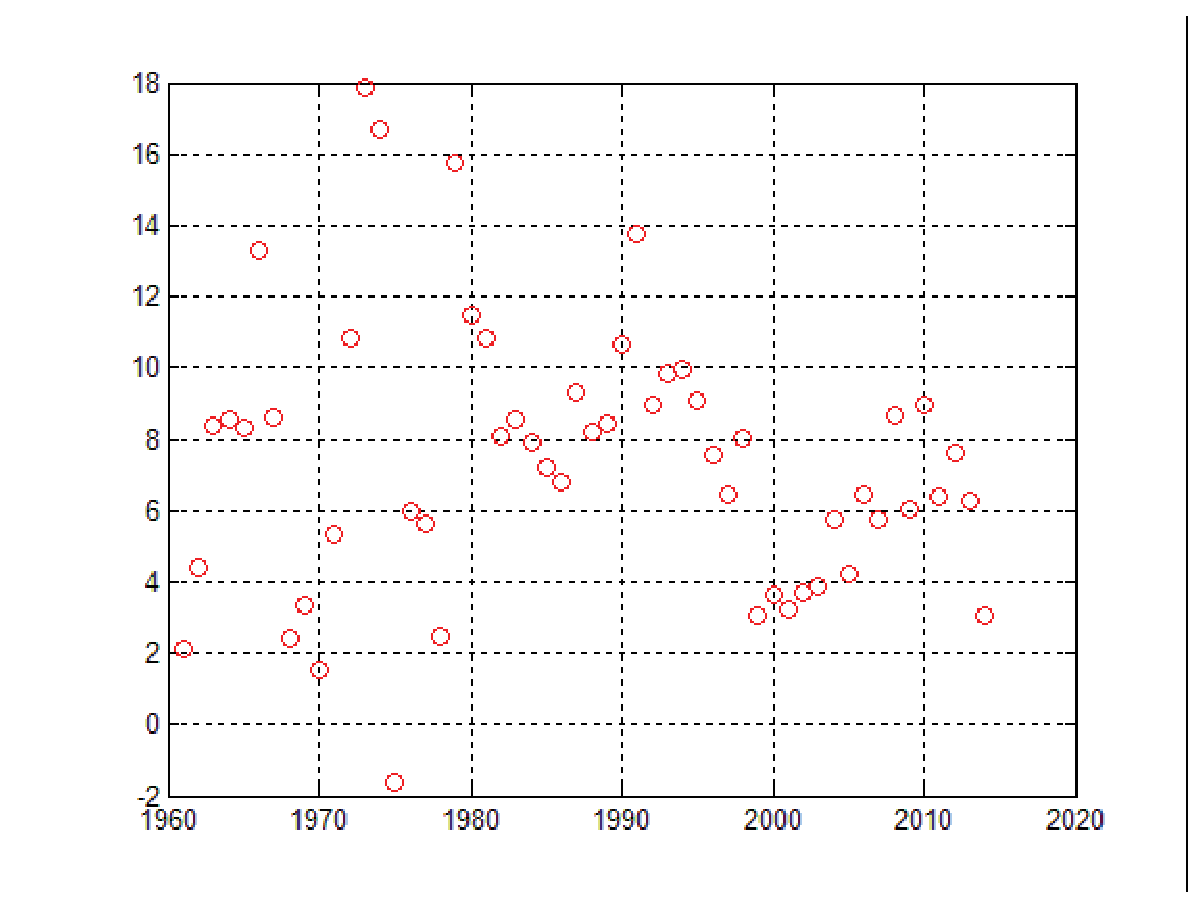
\includegraphics[width=11cm]{inflationGDPDeflator.eps}
\caption{Inflation, GDP deflator of India} \label{fig:inflationGDPDeflator}
\end{figure}

\begin{Theorem}
Water productivity is calculated as GDP in constant prices divided by annual total water withdrawal.
\footnote{The World Bank. 
Water productivity. 
\emph{World Development Indicators}, 
December 2015.}
\label{thm:waterProductivity}
\end{Theorem}

Table \ref{tab:waterProductivity}
\footnote{The World Bank. 
Water productivity. 
\emph{World Development Indicators}, 
December 2015.}
is on water productivity on India.
\begin{table}[]
\centering
\begin{tabular}{@{}cc|cc@{}}
\toprule
Year & \begin{tabular}[c]{@{}c@{}}Water productivity\\ (constant 2005 US\$ GDP\\ per cubic meter of\\ total freshwater withdrawal)\end{tabular} & Year & Water productivity \\ \midrule
1977 & 0.502009010450901 & 1982 & 0.510462079856866 \\
1987 & 0.574461186551227 & 1992 & 0.746694560746423 \\
2001 & 1.07430530471852 & 2012 & 1.83130887829215 \\
2013 & 1.95765485601753 \\ \bottomrule
\end{tabular}
\caption{Water productivity of India}
\label{tab:waterProductivity}
\end{table}

We use curve-fitting, 
and out put figure \ref{fig:waterProductivity} describes and predicts the water productivity of India in 15 years.

\begin{figure}[]
\small
\centering
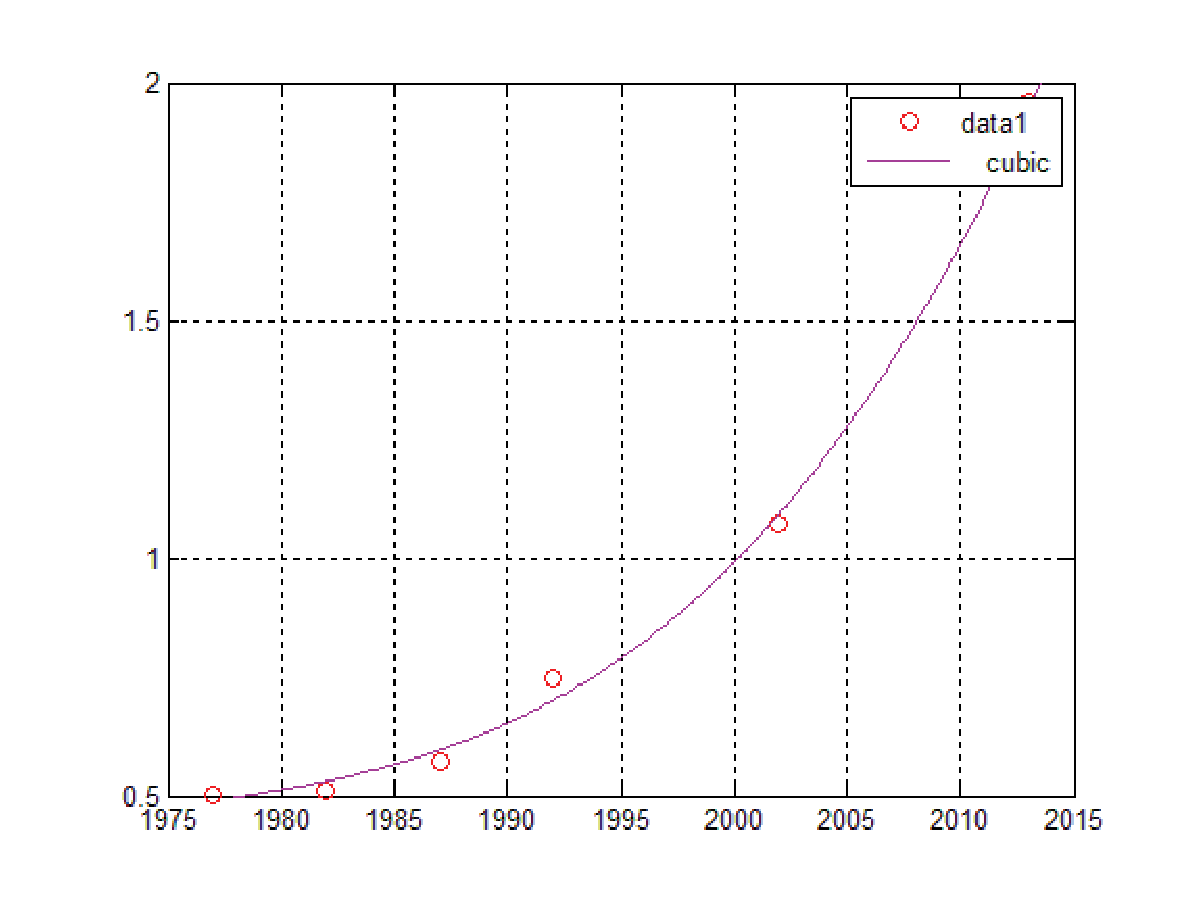
\includegraphics[width=11cm]{waterProductivity.eps}
\caption{Water Productivity of India in 15 years} \label{fig:waterProductivity}
\end{figure}

Since the water productivity of India hasn't changed much in recent 20 years, 
we take water productivity of India $\zeta$ as constant. 
That is $\zeta = 5\hspace{1 ex} US\$ / m^3$.

\item In consideration of basic living needs for water, 
we assign $60.955\hspace{1 ex} m^3/p/yr$ to $\varepsilon$. 
\end{itemize}

\subsection{Grey Forecasting Model}

\hspace{1.5 em} Grey theory deals with systems that are characterized by poor information or for which information is lacking.
The section presents a Grey Forecasting Model, 
GM(1,1), 
using a technique that forecast GDP at market prices 
(current US\$) of India in 15 years.

Assume an original data series to be
\begin{equation}
X^{(0)}(k) = {x^0(1), x^0(2), ... , x^0(n)}
\end{equation}

The Accumulated Generation Operation 
( AGO) 
is expressed as
\begin{equation}
X^{(1)}(k) = \sum_{n = 1}^{k} x^0(n)
\end{equation}

The first-order differential equation of GM(1,1) model is then give as
\begin{equation}
\frac{dX^{(1)}}{dT} + aX^{(1)} = b
\label{eq:firstOrderDifferentialEquation}
\end{equation}

The solution for Equation \eqref{eq:firstOrderDifferentialEquation} is
\begin{equation}
\widehat{x}^{(1)}(k) = (x^{(0)}(1) - \frac{b}{a})(1 - e^a)e^{-a(k - 1)}, k = 2,3, ..., n
\end{equation}

Where $x^{(1)}(1) = x^{(0)}(1)$ and the coefficients $a$ and $b$ are called developing and grey input coefficient, 
respectively. 
By least-square method, 
they can be obtained as
\begin{equation}
\binom{a}{b} = (A^TA)^{-1}A^TY_{n}
\end{equation}

Where
\begin{equation}
A = 
\begin{pmatrix}
- \frac{1}{2}( x^{(1)}(1) + x^{(1)}(2) ) & 1 \\ 
- \frac{1}{2}( x^{(1)}(2) + x^{(1)}(3) )  & 1 \\ 
\vdots & \vdots \\ 
- \frac{1}{2}( x^{(1)}(n - 1) + x^{(1)}(n) ) & 1
\end{pmatrix}
\end{equation}

\begin{equation}
Y_{n} = 
\begin{bmatrix}
x^{(0)}(2) \\ 
x^{(0)}(3) \\ 
\vdots \\ 
x^{(0)}(n)
\end{bmatrix}
\end{equation}

\textbf{Create the function document} 
(see Appendix \ref{lst:greyForecastingModel}).

Table \ref{tab:GDPOfIndia}
\footnote{The World Bank. 
GDP at market prices (current US\$). 
\emph{World Development Indicators}, 
December 2015.}
is on GDP at market prices 
(current US\$) of India.
\begin{table}[]
\centering
\begin{tabular}{@{}cc|cc|cc@{}}
\toprule
Year & \begin{tabular}[c]{@{}c@{}}GDP at market prices\\ (current US\$) \end{tabular} & Year & GDP at market prices & Year & GDP at market prices \\ \midrule
1960 & 37679274491.2745 & 1961 & 39920452403.4524 & 1962 & 42900864969.865 \\
1963 & 49271095508.0955 & 1964 & 57470781032.781 & 1965 & 60599264111.7178 \\
1966 & 46669801600 & 1967 & 51014155360 & 1968 & 54016411986.6667 \\
1969 & 59472993626.6667 & 1970 & 63517182000 & 1971 & 68532271313.2286 \\
1972 & 72716595884.3124 & 1973 & 87014945186.3156 & 1974 & 101271489826.241 \\
1975 & 100199514365.231 & 1976 & 104518118776.804 & 1977 & 123617837582.482 \\
1978 & 139708688961.553 & 1979 & 155674337010.019 & 1980 & 189594121351.874 \\
1981 & 196883474523.345 & 1982 & 204234366470.486 & 1983 & 222090283347.207 \\
1984 & 215878233650.679 & 1985 & 236589100981.279 & 1986 & 253352444883.275 \\
1987 & 283926977522.458 & 1988 & 301790951204.236 & 1989 & 301233728792.841 \\
1990 & 326608014285.316 & 1991 & 274842161318.346 & 1992 & 293262722482.422 \\
1993 & 284194018792.066 & 1994 & 333014993709.73 & 1995 & 366600193391.349 \\
1996 & 399787263892.645 & 1997 & 423160799040.86 & 1998 & 428740690379.961 \\
1999 & 466866720520.974 & 2000 & 476609148165.173 & 2001 & 493954161367.563 \\
2002 & 523968381476.715 & 2003 & 618356467437.027 & 2004 & 721584805204.777 \\
2005 & 834214699568.14 & 2006 & 949116769619.215 & 2007 & 1238699170077.86 \\
2008 & 1224097069460.46 & 2009 & 1365371474048.93 & 2010 & 1708458876830.18 \\
2011 & 1835814449585.35 & 2012 & 1831781515472.09 & 2013 & 1861801615477.85 \\
2014 & 2048517438873.54 & 2015 \\
\bottomrule
\end{tabular}
\caption{GDP at market prices of India}
\label{tab:GDPOfIndia}
\end{table}

\textbf{Run Result}

$G = 133045.15$

which $G = 133045.15 \times 10^8\hspace{1 ex} US\$$ is estimate of GDP at market prices of India in 2031.

Figure \ref{fig:GDPOfIndiaIn15Years} describes and predicts the GDP of India in 15 years.

\begin{figure}[]
\small
\centering
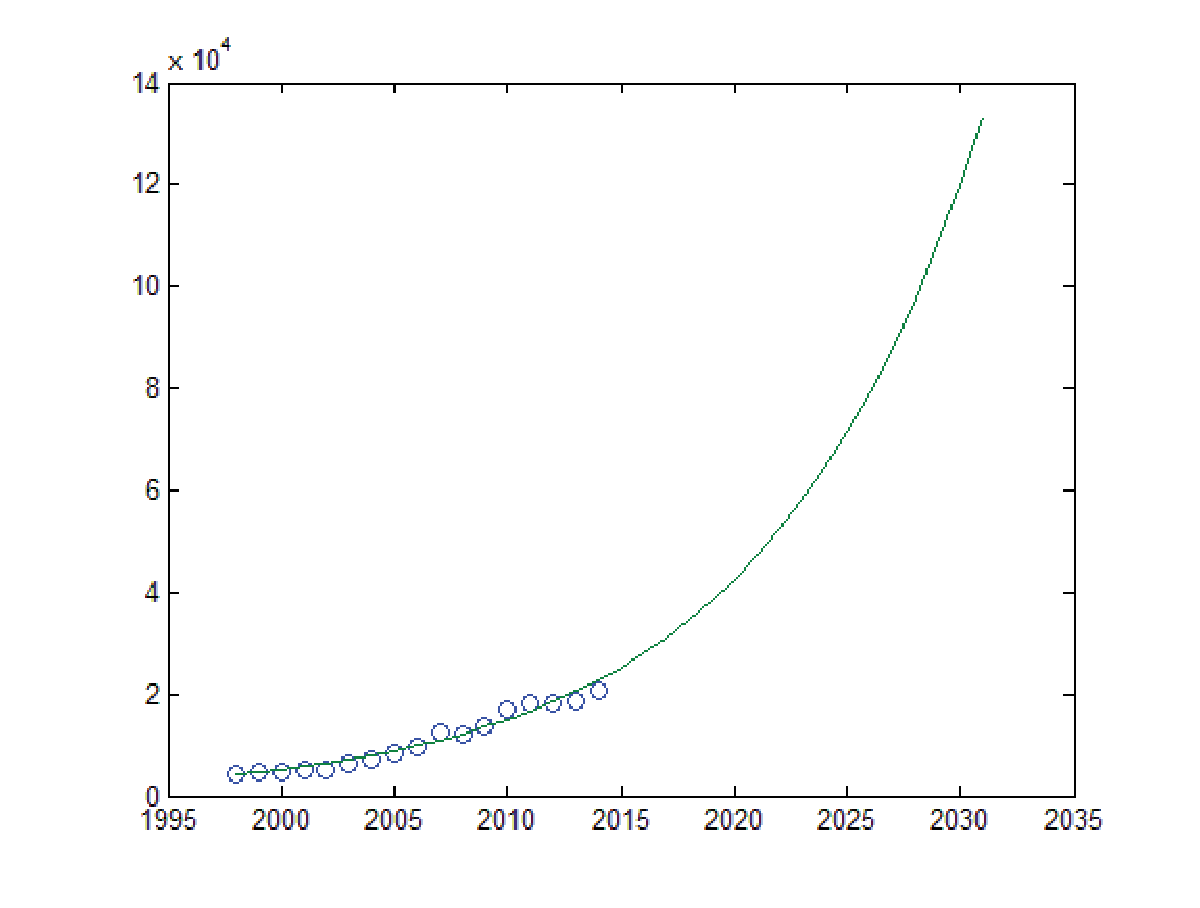
\includegraphics[width=11cm]{greyForecastingModel.eps}
\caption{GDP at market prices of India in 15 years} \label{fig:GDPOfIndiaIn15Years}
\end{figure}

\subsection{Logistic Retarded Growth Model}

\hspace{1.5 em} Because of the inhibition of factors such as resource and environment population growth, 
population increases slow down as the population approaches a certain quantity.
We assume that the growth rate of population is decreasing function of $x$.
Set
\begin{equation}
r(x) = r( 1 - \frac{x}{x_{m}} )
\end{equation}
Which $r$ is inherent growth rate 
( when $x$ is small), 
$x_{m}$ is population carrying capacity 
( the maximum population size that the resource and environment can sustain indefinitely),
so we have the following differential equation: 
\begin{equation}
\begin{cases}
\frac{dx}{dt} = r \cdot x ( 1 - \frac{x}{x_{m}} ) \\
x(0) = x_{0}  
\end{cases}
\end{equation}

\textbf{Create the function document} 
(see Appendix \ref{lst:logisticRetardedGrowthModel}).

Table \ref{tab:populationOfIndia}
\footnote{The World Bank. 
Population, total. 
\emph{World Development Indicators}, 
December 2015.}
is on the population of India.
\begin{table}[]
\centering
\begin{tabular}{@{}cc|cc|cc@{}}
\toprule
Year & Population & Year & Population & Year & Population \\ \midrule
1960 & 449661874 & 1961 & 458691457 & 1962 & 468054145 \\
1963 & 477729958 & 1964 & 487690114 & 1965 & 497920270 \\
1966 & 508402908 & 1967 & 519162069 & 1968 & 530274729 \\
1969 & 541844848 & 1970 & 553943226 & 1971 & 566605402 \\
1972 & 579800632 & 1973 & 593451889 & 1974 & 607446519 \\
1975 & 621703641 & 1976 & 636182810 & 1977 & 650907559 \\
1978 & 665936435 & 1979 & 681358553 & 1980 & 697229745 \\
1981 & 713561406 & 1982 & 730303461 & 1983 & 747374856 \\
1984 & 764664278 & 1985 & 782085127 & 1986 & 799607235 \\
1987 & 817232241 & 1988 & 834944397 & 1989 & 852736160 \\
1990 & 870601776 & 1991 & 888513869 & 1992 & 906461358 \\
1993 & 924475633 & 1994 & 942604211 & 1995 & 960874982 \\
1996 & 979290432 & 1997 & 997817250 & 1998 & 1016402907 \\
1999 & 1034976626 & 2000 & 1053481072 & 2001 & 1071888190 \\
2002 & 1090189358 & 2003 & 1108369577 & 2004 & 1126419321 \\
2005 & 1144326293 & 2006 & 1162088305 & 2007 & 1179685631 \\
2008 & 1197070109 & 2009 & 1214182182 & 2010 & 1230984504 \\
2011 & 1247446011 & 2012 & 1263589639 & 2013 & 1279498874 \\
2014 & 1295291543 & 2015 & & & \\ \bottomrule
\end{tabular}
\caption{Population of India}
\label{tab:populationOfIndia}
\end{table}

\textbf{Run Result}

$a = 29.2225 \quad 0.0280281$

$y1 = 16.6703$

Which $a_{1}$ and $a_{2}$ represent $x_{m}$ and $r$
in $x(t) = \frac{x_{m}}{1+(\frac{x_{m}}{x_{0}}-1) \cdot e^{-r \cdot t}}$
respectively, 
while $y1 = 1.66703\hspace{1 ex} billion$ is estimate of the population of India in 2031.

Figure \ref{fig:populationOfIndiaIn15Years} describes and predicts the population of India in 15 years.

\begin{figure}[]
\small
\centering
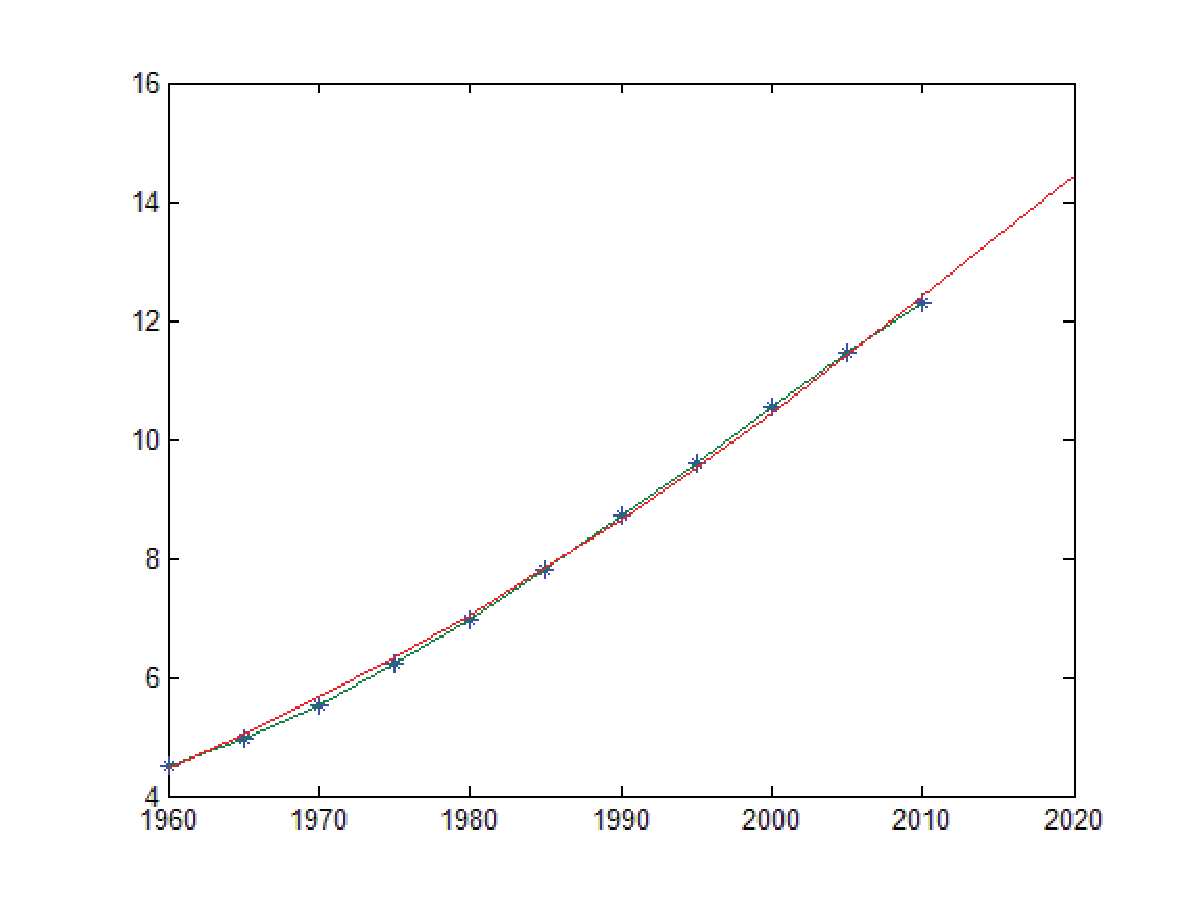
\includegraphics[width=11cm]{logisticRetardedGrowthModel.eps}
\caption{Population of India in 15 years} \label{fig:populationOfIndiaIn15Years}
\end{figure}

\subsection{Results Of Prediction Model}

\hspace{1.5 em} For constant-price GDP $G_{let}$

\begin{Lemma}
\begin{equation}
G_{let} = \frac{G}{\eta + 1}
\end{equation}
\end{Lemma}

when $G = 133045.15 \times 10^8$, 
and $2\% \leqslant \eta \leqslant 10\%$, 
we have $G_{let} = \frac{133045.15 \times 10^8}{\eta +1}$, 
thus $1.2095014 \times 10^{13} \leqslant G_{let} \leqslant 1.3043642 \times 10^{13}$

\begin{Lemma}
\begin{equation}
\omega = \frac{G_{let}}{\zeta}
\end{equation}
\end{Lemma}

When $\zeta = 5\hspace{1 ex} US\$ / m^3$ as we mentioned before, 
we have 
\begin{equation}
2491.0028\hspace{1 ex} km^3/yr \leqslant \varphi + \omega \leqslant 2608.7284\hspace{1 ex} km^3/yr
\end{equation}


Domestic water demand is
\begin{equation}
\theta \cdot \varepsilon = 16.6703 \times 10^8 \cdot 60.955 = 101.6138137\hspace{1 ex} km^3/yr
\end{equation}

Like Equation \ref{eq:relation}, 
we have
\begin{equation}
\rho = from\hspace{1 ex} 23.02\%\hspace{1 ex} to\hspace{1 ex} 24.83\%
\end{equation}

Given the water resources utilization level and water resources exploitation extent basically unchanged, 
with the population dramatically increasing and huge consumption for GDP growth in 15 years, 
the relation between water supply and demand will drop from 78.887\% to about 24\%, 
which means that water scarcity becomes even tense. 
Even if in an ideal world, 
water resources exploitation extent increases to 100\%, 
the relation between water supply and demand is merely 45\%, 
which cannot meet the needs for water of its citizens, 
and leads to massively shortage of water.

\subsection{Impact On the Lives Of the Citizens Of India}

\hspace{1.5 em} Apart from inadequate supply of water, 
27\% of the villages and 4\% to 6\% urban population in India lack access to drinking water. 
There is a genuine concern about the quality of water, 
which is severely affecting the health. 
It is reported that over 70\% of the water consumed by the rural population in India does not meet the WHO standards. 
It has been reported that 80\% of rural illnesses, 
21\% of transmissible diseases and 20\% of deaths among children in the age group of 5 years, 
are directly linked to consumption of unsafe water. 

In 2031, 
a large number of people are suffering from fluorosis after consuming water containing more than 1.5 ppm fluoride. 
Poor sanitation both in rural and urban areas, is another reason for pollution of drinking water sources. 
Nitrates and harmful germs from human excreta flow and percolate down to contaminate the water tanks and open wells. 

Most of the well water used for drinking in irrigated areas is polluted. 
Excessive irrigation has also been causing further damage to soil productivity. 
As the water reaching lower layers of soil and the salts present in this region are dissolved in water. 
Subsequently, these salts come to the top soil through capillary action. 
Such soils with high concentrations turn into sodic wastelands, 
unfit for agricultural production. 
As the people living in these villages are helplessly consuming such hard water, the incidences of illnesses are high.

\section{The intervention plan}

\hspace{1.5 em} Since the total availability of water resources is invariable, 
with one central task of India is at developing economy, 
boosting GDP should never stagnate. 
Consumption for GDP growth is essential; 
domestic water is also requisite; 
growth of population is difficult to control. 
Under such circumstances, 
a sensible intervention plan to remit water scarcity is to sewage disposal. 
We find that the investigation of the governments makes a great difference to development of sewage disposal.

In this section, 
we establish the Sewage Disposal Price System, 
Sewage Disposal Quantity System and Psychological Prediction Model with proportion of investment of the governments as parameters.

\subsection{Sewage Disposal Model}

\hspace{1.5 em} Parameters involved in this model are shown as follows: 

\begin{itemize}
\item Sewage disposal price per unit volume $p\hspace{1 ex}US\$/m^3$
\item The proportion of investment of the government $x$
\item The volume of sewage treated per year $v$
\item For a sewage plant, 
its construction capital to sewage treated quantity per day ratio is approximately constant, 
which defined as $m$. 
\item We assume that the lifetime of a sewage is 20 years. 
To attract social capitals, 
we need to provide investors with yield $r$. 
The common industry yield is from 8\% to 12\%. 
Here, 
we assign 10\% to it.
\item The daily operating costs of a sewage plant $z = 0.1\hspace{1 ex}US\$/m^3$
\end{itemize}

So, 
the ideal prediction model of $P$ is
\begin{equation}
p = \frac{m}{20} \cdot (1 - x) \cdot r + z
\end{equation}

\subsection{Phychological Prediction Model}

\hspace{1.5 em} Meanwhile, 
we assume that sewage plant investors are rational. 
That is they pursue interest. 
As long as the government invests more, 
the investors invest more. 
We establish Psychological Prediction Model with $x$ and $v$:
\begin{equation}
v = \beta \cdot (1 - e^{-x^2})
\end{equation}

Figure \ref{fig:phychologicalPredictionModel} describes the relationship between $x$ and $v$, 
also $x$ and $p$.

\begin{figure}[]
\small
\centering
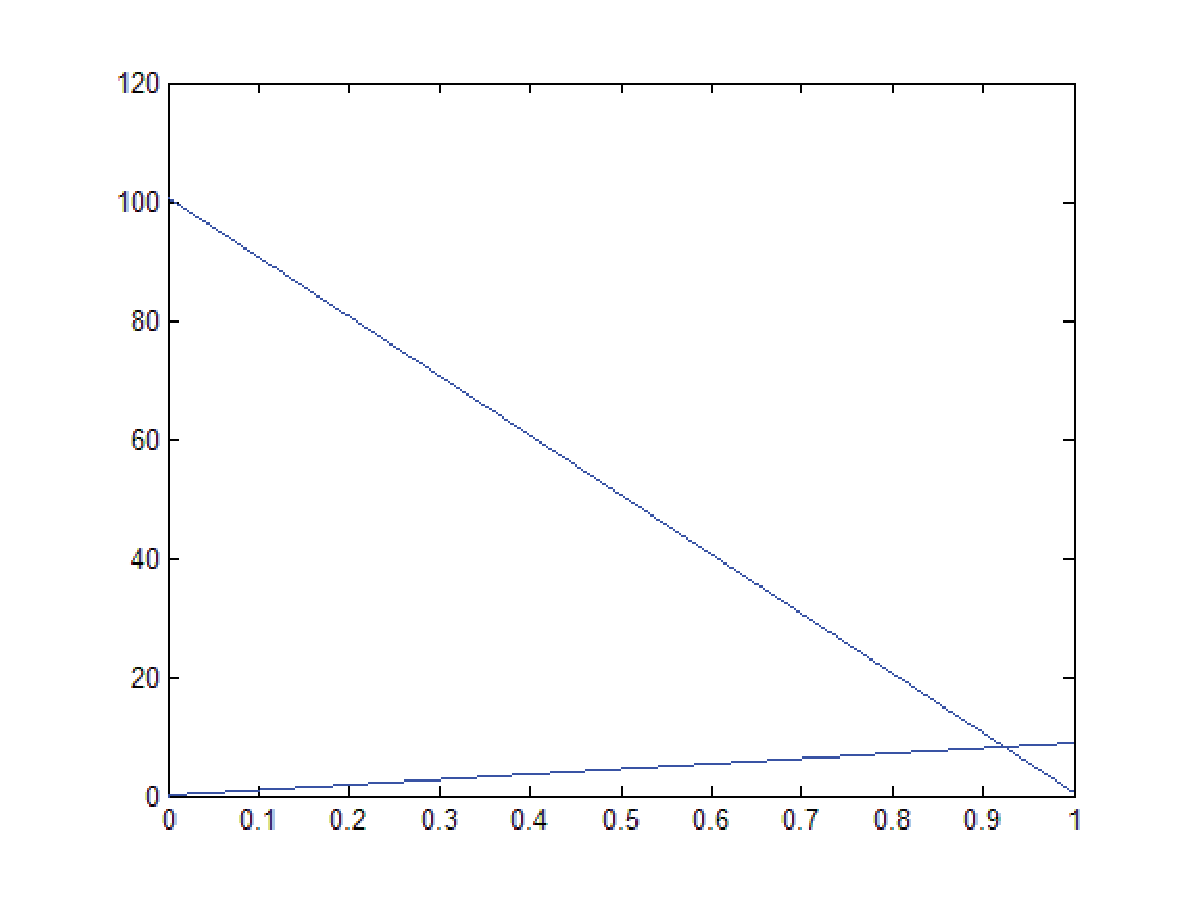
\includegraphics[width=11cm]{phychologicalPredictionModel.eps}
\caption{Phychological Prediction Model} \label{fig:phychologicalPredictionModel}
\end{figure}

By comprehensive evaluation of Figure \ref{fig:phychologicalPredictionModel}, 
to make $p$ as small as possible, 
while $v$ as large as possible, 
$0.7 \leqslant x \leqslant 0.9$, 
which means the most optimal proportion of investment of the government is between 70\% to 90\%.

\subsection{Analysis Of the Intervention Plan}

\hspace{1.5 em} In this section, 
we describe the impact of our intervention plan on India, 
which is also the strengths and weaknesses of the plan.

\begin{itemize}

\item \textbf{Strengths} \\

\emph{Environment}

Sewage plants collect wastewater, 
make the wastewater meet the emission standard, 
and recycle it. 
Its series of treatments not only increase the utilization of freshwater, 
but also reduce the pollutant, 
which have an important protection for water, 
soil and air resources. 

Sewage plants protect groundwater resources from polluting for wastewater seeps into the ground in most cases. They also protect soil and plants downstream. 

\item \textbf{Weaknesses} \\

\emph{Environment}

At present, 
sewage treatment is complicated. 
It needs sewage pump, 
wastewater treatment facility-integral equipment which will produce noise pollution. 
The noise pollution from sewage plants may reduce quality of life. 

In another aspect, 
sewage has complex origins and multiple elements, 
mainly including sulphur compounds such as $H_{2}S$, 
$SO_{2}$, 
mercaptan and thiophene; 
nitrogen compounds such as $NH_{3}$ and amine; 
hydrocarbon compound such as alkane, 
olefin and arene; 
oxygen-contained compounds such as alcohol and aldehyde. 
These gases and vapours will spread air pollution.

\emph{Economy}

In our Sewage Disposal Model, 
sewage treatment is mainly funded by society, 
while the investment of government plays a supplementary role. 
Sewage treatment is not profitable, 
so sewage project is always at a loss.

\end{itemize}

\section{Water Scarcity Prediction Model}

\hspace{1.5 em} We use the recognized water scarcity warning line, 
annual per capita renewable freshwater availability is 1,000 cubic meters, 
as standard. 
We convert annual per capita freshwater availability to relation between water supply and demand, 
that means when $\rho$ reaches over 63.1\%, 
the ability of India to provide clean water to meet the minimum needs for water.

We assume that sewage plants in India process 90\% to 100\% sewage.  
According to our intervention plan, 
we have
\begin{equation}
\rho = \frac{\gamma}{ \frac{G_{let}}{(\eta + 1) \cdot \zeta + \varepsilon \cdot \theta} } \geqslant 63.1\%
\end{equation}

We integrate data into Table \ref{tab:demandOfWater}. 
\begin{table}[]
\centering
\begin{tabular}{@{}cccc@{}}
\toprule
Year & GDP & Population & Demand Of Water \\ \midrule
1995 & 366600193391 & 960874982 & 136.098 \\
2000 & 476609148165 & 1053481072 & 195.841 \\
2005 & 834214699568 & 1144326293 & 291.595 \\
2010 & 1708458876830 & 1230984504 & 448.738 \\
2015 & 3448924517813 & 1341058433 & 708.881 \\
2020 & 5796817144582 & 1443169380 & 1142.000 \\
2025 & 9743063043035 & 1545456036 & 1865.738 \\
2030 & 11992172785919 & 1646920019 & 2280.857 \\
\bottomrule
\end{tabular}
\caption{Demand of Water in India in 15 years}
\label{tab:demandOfWater}
\end{table}

\subsection{Results Of Water Scarcity Prediction Model}

\hspace{1.5 em} In this section, 
we explain water scarcity in India with no intervention, 
our intervention, 
and in an ideal situation.

\begin{itemize}

\item \textbf{With no intervention} \\

Like Equation \ref{eq:supply}, 
$\gamma = 600.578\hspace{1 ex}km^3/yr$, 
so, the maximum demand for water is $951.787\hspace{1 ex}km^3/yr$. 
According to Table \ref{tab:demandOfWater}, 
we estimate that water scarcity will occur around 2017. 

\item \textbf{With our intervention plan} \\

$\beta$ tends be 0, 
so $\gamma = 614.5776\hspace{1 ex}km^3/yr$, 
the maximum demand for water is $973.974\hspace{1 ex}km^3/yr$. 
According to Table \ref{tab:demandOfWater}, 
we estimate that water scarcity will occur around 2018. 

\item \textbf{Best-case scenario}

$\beta$ tends to be 0, 
while $\lambda$ is tend to be 100\%, 
so $\gamma = 1146.6\hspace{1 ex}km^3/yr$. 
so, the maximum demand for water is $1817.115\hspace{1 ex}km^3/yr$. 
According to Table \ref{tab:demandOfWater}, 
we estimate that water scarcity will occur around 2024. 

\end{itemize}

Considering backward technique of sewage treatment and huge amount of sewage in India, 
there is no doubt that sewage disposal is a feasible scheme at present. 
Our Sewage Disposal Model learns from sustainable strategy, 
aiming at the least capital from the government and the most effective wastewater treatment, 
mitigating water scarcity.

Using our intervention plan, 
water scarcity will be postponed 1 year after no intervention. 
In an ideal situation, 
it will be postponed 7 years after no intervention. 
Thus, 
it proves that our intervention plan is valuable.

In conclusion, 
India can become less susceptible to waters scarcity. 
It is a pity that water become a critical issue sooner or later.

\section{Conclusions}

\hspace{1.5 em}In this section, 
we detail the strengths and weaknesses of our models.

\subsection{Evaluation Of Grey Forecasting Model}

\begin{itemize}

\item \textbf{Strengths} \\

Grey Forecasting Model needs small amounts of data, 
whose prediction is relatively accurate. 
The sample data doesn't need regularity of distribution. 
The model is simple in computation and checked conveniently. 

Grey Forecasting Model is applied to medium long term prediction. 
It has its superiority in predicting GDP.

\item \textbf{Weaknesses} \\

With enough data, 
the prediction is an exact science, 
while in the other way, 
it has an accuracy deviation.

In our paper, 
we have no comprehensive and perfect statistics on data of India. 
Thus our results produce some error inevitably.

\end{itemize}

\subsection{Evaluation Of Logistic Retarded Growth Model}

\begin{itemize}

\item \textbf{Strengths} \\

We use Logistic Model for prediction of population, 
and we also take the inhibition into account. 
The prediction is in line with objective laws and credible for the authoritative history data.

\item \textbf{Weaknesses} \\

The Logistic Model neglects some uncontrollable influences from policy, 
such as the birth control in China. 
As a result, 
the prediction is about population explosion without intervention, 
whose figures increase dramatically.

\end{itemize}

\subsection{Evaluation Of Psychological Prediction Model}

\begin{itemize}

\item \textbf{Strengths} \\

Psychological Prediction Model is estimation for social investors' investment psychology. 
It analyses the possibility of social investment under the change of the government's fund. 
It's an effective discretization algorithm for psychological change.

\item \textbf{Weaknesses} \\

Psychological Prediction Model is based on the investors for-profit purpose, 
neglecting purpose for public interest or advertising.

\end{itemize}

\newpage
\bibliographystyle{IEEEtran}
\begin{thebibliography}{}
\bibitem{1} A. Tsoularis, J. Wallace, Analysis of logistic growth models, \emph{Mathematical Biosciences}, Volume 179, Issue 1, July?August 2002, Pages 21-55, ISSN 0025-5564.
\bibitem{2} James H. Matis, Thomas R. Kiffe, On stochastic logistic population growth models with immigration and multiple births, \emph{Theoretical Population Biology}, Volume 65, Issue 1, February 2004, Pages 89-104, ISSN 0040-5809.
\bibitem{3} Witold Kwasnicki, Logistic growth of the global economy and competitiveness of nations, \emph{Technological Forecasting and Social Change}, Volume 80, Issue 1, January 2013, Pages 50-76, ISSN 0040-1625.
\bibitem{4} Zwe-Lee Gaing, Rong-Ceng Leon, Optimal grey topological predicting approach to short-term load forecasting in power system, \emph{Power Engineering Society, IEEE Summer Meeting}, 2002, 10.1109/PESS.2002.1043533.
\end{thebibliography}

\newpage
\begin{appendices}

\section{Grey Forecasting Model}
\hspace{1.5 em} Here is the function definition programme for we used in our Grey Forecasting Model as follow. \\

\textbf{\textcolor[rgb]{0.98,0.00,0.00}{Input Matlab source:}}
\lstinputlisting[language=Matlab]{./code/greyForecastingModel.m}
\label{lst:greyForecastingModel}

\section{Logistic Retarded Growth Model}

\hspace{1.5 em} Here is the function definition programme for we used in our Logistic Retarded Growth Model as follow. \\

\textbf{\textcolor[rgb]{0.98,0.00,0.00}{Input Matlab source:}}
\lstinputlisting[language=Matlab]{./code/logisticRetardedGrowthModel.m}
\label{lst:logisticRetardedGrowthModel}

\end{appendices}

\end{document}